% Options for packages loaded elsewhere
\PassOptionsToPackage{unicode}{hyperref}
\PassOptionsToPackage{hyphens}{url}
%
\documentclass[
]{article}
\usepackage{amsmath,amssymb}
\usepackage{iftex}
\ifPDFTeX
  \usepackage[T1]{fontenc}
  \usepackage[utf8]{inputenc}
  \usepackage{textcomp} % provide euro and other symbols
\else % if luatex or xetex
  \usepackage{unicode-math} % this also loads fontspec
  \defaultfontfeatures{Scale=MatchLowercase}
  \defaultfontfeatures[\rmfamily]{Ligatures=TeX,Scale=1}
\fi
\usepackage{lmodern}
\ifPDFTeX\else
  % xetex/luatex font selection
\fi
% Use upquote if available, for straight quotes in verbatim environments
\IfFileExists{upquote.sty}{\usepackage{upquote}}{}
\IfFileExists{microtype.sty}{% use microtype if available
  \usepackage[]{microtype}
  \UseMicrotypeSet[protrusion]{basicmath} % disable protrusion for tt fonts
}{}
\makeatletter
\@ifundefined{KOMAClassName}{% if non-KOMA class
  \IfFileExists{parskip.sty}{%
    \usepackage{parskip}
  }{% else
    \setlength{\parindent}{0pt}
    \setlength{\parskip}{6pt plus 2pt minus 1pt}}
}{% if KOMA class
  \KOMAoptions{parskip=half}}
\makeatother
\usepackage{xcolor}
\usepackage[margin=1in]{geometry}
\usepackage{color}
\usepackage{fancyvrb}
\newcommand{\VerbBar}{|}
\newcommand{\VERB}{\Verb[commandchars=\\\{\}]}
\DefineVerbatimEnvironment{Highlighting}{Verbatim}{commandchars=\\\{\}}
% Add ',fontsize=\small' for more characters per line
\usepackage{framed}
\definecolor{shadecolor}{RGB}{248,248,248}
\newenvironment{Shaded}{\begin{snugshade}}{\end{snugshade}}
\newcommand{\AlertTok}[1]{\textcolor[rgb]{0.94,0.16,0.16}{#1}}
\newcommand{\AnnotationTok}[1]{\textcolor[rgb]{0.56,0.35,0.01}{\textbf{\textit{#1}}}}
\newcommand{\AttributeTok}[1]{\textcolor[rgb]{0.13,0.29,0.53}{#1}}
\newcommand{\BaseNTok}[1]{\textcolor[rgb]{0.00,0.00,0.81}{#1}}
\newcommand{\BuiltInTok}[1]{#1}
\newcommand{\CharTok}[1]{\textcolor[rgb]{0.31,0.60,0.02}{#1}}
\newcommand{\CommentTok}[1]{\textcolor[rgb]{0.56,0.35,0.01}{\textit{#1}}}
\newcommand{\CommentVarTok}[1]{\textcolor[rgb]{0.56,0.35,0.01}{\textbf{\textit{#1}}}}
\newcommand{\ConstantTok}[1]{\textcolor[rgb]{0.56,0.35,0.01}{#1}}
\newcommand{\ControlFlowTok}[1]{\textcolor[rgb]{0.13,0.29,0.53}{\textbf{#1}}}
\newcommand{\DataTypeTok}[1]{\textcolor[rgb]{0.13,0.29,0.53}{#1}}
\newcommand{\DecValTok}[1]{\textcolor[rgb]{0.00,0.00,0.81}{#1}}
\newcommand{\DocumentationTok}[1]{\textcolor[rgb]{0.56,0.35,0.01}{\textbf{\textit{#1}}}}
\newcommand{\ErrorTok}[1]{\textcolor[rgb]{0.64,0.00,0.00}{\textbf{#1}}}
\newcommand{\ExtensionTok}[1]{#1}
\newcommand{\FloatTok}[1]{\textcolor[rgb]{0.00,0.00,0.81}{#1}}
\newcommand{\FunctionTok}[1]{\textcolor[rgb]{0.13,0.29,0.53}{\textbf{#1}}}
\newcommand{\ImportTok}[1]{#1}
\newcommand{\InformationTok}[1]{\textcolor[rgb]{0.56,0.35,0.01}{\textbf{\textit{#1}}}}
\newcommand{\KeywordTok}[1]{\textcolor[rgb]{0.13,0.29,0.53}{\textbf{#1}}}
\newcommand{\NormalTok}[1]{#1}
\newcommand{\OperatorTok}[1]{\textcolor[rgb]{0.81,0.36,0.00}{\textbf{#1}}}
\newcommand{\OtherTok}[1]{\textcolor[rgb]{0.56,0.35,0.01}{#1}}
\newcommand{\PreprocessorTok}[1]{\textcolor[rgb]{0.56,0.35,0.01}{\textit{#1}}}
\newcommand{\RegionMarkerTok}[1]{#1}
\newcommand{\SpecialCharTok}[1]{\textcolor[rgb]{0.81,0.36,0.00}{\textbf{#1}}}
\newcommand{\SpecialStringTok}[1]{\textcolor[rgb]{0.31,0.60,0.02}{#1}}
\newcommand{\StringTok}[1]{\textcolor[rgb]{0.31,0.60,0.02}{#1}}
\newcommand{\VariableTok}[1]{\textcolor[rgb]{0.00,0.00,0.00}{#1}}
\newcommand{\VerbatimStringTok}[1]{\textcolor[rgb]{0.31,0.60,0.02}{#1}}
\newcommand{\WarningTok}[1]{\textcolor[rgb]{0.56,0.35,0.01}{\textbf{\textit{#1}}}}
\usepackage{graphicx}
\makeatletter
\def\maxwidth{\ifdim\Gin@nat@width>\linewidth\linewidth\else\Gin@nat@width\fi}
\def\maxheight{\ifdim\Gin@nat@height>\textheight\textheight\else\Gin@nat@height\fi}
\makeatother
% Scale images if necessary, so that they will not overflow the page
% margins by default, and it is still possible to overwrite the defaults
% using explicit options in \includegraphics[width, height, ...]{}
\setkeys{Gin}{width=\maxwidth,height=\maxheight,keepaspectratio}
% Set default figure placement to htbp
\makeatletter
\def\fps@figure{htbp}
\makeatother
\setlength{\emergencystretch}{3em} % prevent overfull lines
\providecommand{\tightlist}{%
  \setlength{\itemsep}{0pt}\setlength{\parskip}{0pt}}
\setcounter{secnumdepth}{-\maxdimen} % remove section numbering
\newlength{\cslhangindent}
\setlength{\cslhangindent}{1.5em}
\newlength{\csllabelwidth}
\setlength{\csllabelwidth}{3em}
\newlength{\cslentryspacingunit} % times entry-spacing
\setlength{\cslentryspacingunit}{\parskip}
\newenvironment{CSLReferences}[2] % #1 hanging-ident, #2 entry spacing
 {% don't indent paragraphs
  \setlength{\parindent}{0pt}
  % turn on hanging indent if param 1 is 1
  \ifodd #1
  \let\oldpar\par
  \def\par{\hangindent=\cslhangindent\oldpar}
  \fi
  % set entry spacing
  \setlength{\parskip}{#2\cslentryspacingunit}
 }%
 {}
\usepackage{calc}
\newcommand{\CSLBlock}[1]{#1\hfill\break}
\newcommand{\CSLLeftMargin}[1]{\parbox[t]{\csllabelwidth}{#1}}
\newcommand{\CSLRightInline}[1]{\parbox[t]{\linewidth - \csllabelwidth}{#1}\break}
\newcommand{\CSLIndent}[1]{\hspace{\cslhangindent}#1}
\ifLuaTeX
  \usepackage{selnolig}  % disable illegal ligatures
\fi
\IfFileExists{bookmark.sty}{\usepackage{bookmark}}{\usepackage{hyperref}}
\IfFileExists{xurl.sty}{\usepackage{xurl}}{} % add URL line breaks if available
\urlstyle{same}
\hypersetup{
  pdftitle={Parkinson data - I},
  pdfauthor={Giovanni Saraceno},
  hidelinks,
  pdfcreator={LaTeX via pandoc}}

\title{Parkinson data - I}
\author{Giovanni Saraceno}
\date{}

\begin{document}
\maketitle

{
\setcounter{tocdepth}{2}
\tableofcontents
}
\begin{Shaded}
\begin{Highlighting}[]
\FunctionTok{library}\NormalTok{(tidyverse)}
\FunctionTok{library}\NormalTok{(dplyr)}
\FunctionTok{library}\NormalTok{(ggplot2)}
\end{Highlighting}
\end{Shaded}

We consider the data set related to the study in Tsanas et al. (2009).
Data can be found at
\href{https://\%20archive.ics.uci.edu/\%20ml/\%20datasets/\%20Parkinsons+Telemonitoring}{https://
archive.ics.uci.edu/ ml/ datasets/ Parkinsons+Telemonitoring}.

We start loading the data.

\begin{Shaded}
\begin{Highlighting}[]
\NormalTok{dat }\OtherTok{\textless{}{-}} \FunctionTok{read.csv}\NormalTok{(}\StringTok{\textquotesingle{}parkinsons\_updrs.data\textquotesingle{}}\NormalTok{, }\AttributeTok{he =} \ConstantTok{TRUE}\NormalTok{, }\AttributeTok{sep =} \StringTok{\textquotesingle{},\textquotesingle{}}\NormalTok{)}
\FunctionTok{str}\NormalTok{(dat)}
\end{Highlighting}
\end{Shaded}

\begin{verbatim}
## 'data.frame':    5875 obs. of  22 variables:
##  $ subject.     : int  1 1 1 1 1 1 1 1 1 1 ...
##  $ age          : int  72 72 72 72 72 72 72 72 72 72 ...
##  $ sex          : int  0 0 0 0 0 0 0 0 0 0 ...
##  $ test_time    : num  5.64 12.67 19.68 25.65 33.64 ...
##  $ motor_UPDRS  : num  28.2 28.4 28.7 28.9 29.2 ...
##  $ total_UPDRS  : num  34.4 34.9 35.4 35.8 36.4 ...
##  $ Jitter...    : num  0.00662 0.003 0.00481 0.00528 0.00335 0.00353 0.00422 0.00476 0.00432 0.00496 ...
##  $ Jitter.Abs.  : num  3.38e-05 1.68e-05 2.46e-05 2.66e-05 2.01e-05 ...
##  $ Jitter.RAP   : num  0.00401 0.00132 0.00205 0.00191 0.00093 0.00119 0.00212 0.00226 0.00156 0.00258 ...
##  $ Jitter.PPQ5  : num  0.00317 0.0015 0.00208 0.00264 0.0013 0.00159 0.00221 0.00259 0.00207 0.00253 ...
##  $ Jitter.DDP   : num  0.01204 0.00395 0.00616 0.00573 0.00278 ...
##  $ Shimmer      : num  0.0256 0.0202 0.0168 0.0231 0.017 ...
##  $ Shimmer.dB.  : num  0.23 0.179 0.181 0.327 0.176 0.214 0.445 0.212 0.371 0.31 ...
##  $ Shimmer.APQ3 : num  0.01438 0.00994 0.00734 0.01106 0.00679 ...
##  $ Shimmer.APQ5 : num  0.01309 0.01072 0.00844 0.01265 0.00929 ...
##  $ Shimmer.APQ11: num  0.0166 0.0169 0.0146 0.0196 0.0182 ...
##  $ Shimmer.DDA  : num  0.0431 0.0298 0.022 0.0332 0.0204 ...
##  $ NHR          : num  0.0143 0.0111 0.0202 0.0278 0.0116 ...
##  $ HNR          : num  21.6 27.2 23 24.4 26.1 ...
##  $ RPDE         : num  0.419 0.435 0.462 0.487 0.472 ...
##  $ DFA          : num  0.548 0.565 0.544 0.578 0.561 ...
##  $ PPE          : num  0.16 0.108 0.21 0.333 0.194 ...
\end{verbatim}

\hypertarget{description-of-the-variables}{%
\paragraph{Description of the
variables}\label{description-of-the-variables}}

\begin{itemize}
\tightlist
\item
  subject\# - Integer that uniquely identifies each subject
\item
  \texttt{age} - Subject age
\item
  \texttt{sex} - Subject gender `0' - male, `1' - female
\item
  \texttt{test\_time} - Time since recruitment into the trial. The
  integer part is the number of days since recruitment.
\item
  \texttt{motor\_UPDRS} - Clinician's motor UPDRS score, linearly
  interpolated
\item
  \texttt{total\_UPDRS} - Clinician's total UPDRS score, linearly
  interpolated
\item
  \texttt{Jitter}(\%), \texttt{Jitter(Abs)}, \texttt{Jitter:RAP},
  \texttt{Jitter:PPQ5}, \texttt{Jitter:DDP} - Several measures of
  variation in fundamental frequency
\item
  \texttt{Shimmer}, \texttt{Shimmer(dB)}, \texttt{Shimmer:APQ3},
  \texttt{Shimmer:APQ5}, \texttt{Shimmer:APQ11}, \texttt{Shimmer:DDA} -
  Several measures of variation in amplitude
\item
  \texttt{NHR}, \texttt{HNR} - Two measures of ratio of noise to tonal
  components in the voice
\item
  \texttt{RPDE} - A nonlinear dynamical complexity measure
\item
  \texttt{DFA} - Signal fractal scaling exponent
\item
  \texttt{PPE} - A nonlinear measure of fundamental frequency variation
\end{itemize}

\begin{Shaded}
\begin{Highlighting}[]
\FunctionTok{str}\NormalTok{(dat)}
\end{Highlighting}
\end{Shaded}

\begin{verbatim}
## 'data.frame':    5875 obs. of  22 variables:
##  $ subject.     : int  1 1 1 1 1 1 1 1 1 1 ...
##  $ age          : int  72 72 72 72 72 72 72 72 72 72 ...
##  $ sex          : int  0 0 0 0 0 0 0 0 0 0 ...
##  $ test_time    : num  5.64 12.67 19.68 25.65 33.64 ...
##  $ motor_UPDRS  : num  28.2 28.4 28.7 28.9 29.2 ...
##  $ total_UPDRS  : num  34.4 34.9 35.4 35.8 36.4 ...
##  $ Jitter...    : num  0.00662 0.003 0.00481 0.00528 0.00335 0.00353 0.00422 0.00476 0.00432 0.00496 ...
##  $ Jitter.Abs.  : num  3.38e-05 1.68e-05 2.46e-05 2.66e-05 2.01e-05 ...
##  $ Jitter.RAP   : num  0.00401 0.00132 0.00205 0.00191 0.00093 0.00119 0.00212 0.00226 0.00156 0.00258 ...
##  $ Jitter.PPQ5  : num  0.00317 0.0015 0.00208 0.00264 0.0013 0.00159 0.00221 0.00259 0.00207 0.00253 ...
##  $ Jitter.DDP   : num  0.01204 0.00395 0.00616 0.00573 0.00278 ...
##  $ Shimmer      : num  0.0256 0.0202 0.0168 0.0231 0.017 ...
##  $ Shimmer.dB.  : num  0.23 0.179 0.181 0.327 0.176 0.214 0.445 0.212 0.371 0.31 ...
##  $ Shimmer.APQ3 : num  0.01438 0.00994 0.00734 0.01106 0.00679 ...
##  $ Shimmer.APQ5 : num  0.01309 0.01072 0.00844 0.01265 0.00929 ...
##  $ Shimmer.APQ11: num  0.0166 0.0169 0.0146 0.0196 0.0182 ...
##  $ Shimmer.DDA  : num  0.0431 0.0298 0.022 0.0332 0.0204 ...
##  $ NHR          : num  0.0143 0.0111 0.0202 0.0278 0.0116 ...
##  $ HNR          : num  21.6 27.2 23 24.4 26.1 ...
##  $ RPDE         : num  0.419 0.435 0.462 0.487 0.472 ...
##  $ DFA          : num  0.548 0.565 0.544 0.578 0.561 ...
##  $ PPE          : num  0.16 0.108 0.21 0.333 0.194 ...
\end{verbatim}

\hypertarget{data-cleaning}{%
\paragraph{Data cleaning}\label{data-cleaning}}

\begin{Shaded}
\begin{Highlighting}[]
\NormalTok{dat}\SpecialCharTok{$}\NormalTok{subject. }\OtherTok{\textless{}{-}} \FunctionTok{as.factor}\NormalTok{(dat}\SpecialCharTok{$}\NormalTok{subject.)}
\NormalTok{dat}\SpecialCharTok{$}\NormalTok{sex }\OtherTok{\textless{}{-}} \FunctionTok{ifelse}\NormalTok{(dat}\SpecialCharTok{$}\NormalTok{sex }\SpecialCharTok{==} \DecValTok{1}\NormalTok{, }\StringTok{\textquotesingle{}F\textquotesingle{}}\NormalTok{, }\StringTok{\textquotesingle{}M\textquotesingle{}}\NormalTok{)}
\NormalTok{dat}\SpecialCharTok{$}\NormalTok{sex }\OtherTok{\textless{}{-}} \FunctionTok{as.factor}\NormalTok{(dat}\SpecialCharTok{$}\NormalTok{sex)}
\end{Highlighting}
\end{Shaded}

\hypertarget{descriptive-analysis}{%
\paragraph{Descriptive analysis}\label{descriptive-analysis}}

Let's have a look at a brief descriptive summary of all the variables

\begin{Shaded}
\begin{Highlighting}[]
\FunctionTok{summary}\NormalTok{(dat)}
\end{Highlighting}
\end{Shaded}

\begin{verbatim}
##     subject.         age       sex        test_time        motor_UPDRS    
##  29     : 168   Min.   :36.0   F:1867   Min.   : -4.263   Min.   : 5.038  
##  35     : 165   1st Qu.:58.0   M:4008   1st Qu.: 46.847   1st Qu.:15.000  
##  41     : 165   Median :65.0            Median : 91.523   Median :20.871  
##  7      : 161   Mean   :64.8            Mean   : 92.864   Mean   :21.296  
##  34     : 161   3rd Qu.:72.0            3rd Qu.:138.445   3rd Qu.:27.596  
##  5      : 156   Max.   :85.0            Max.   :215.490   Max.   :39.511  
##  (Other):4899                                                             
##   total_UPDRS      Jitter...         Jitter.Abs.          Jitter.RAP      
##  Min.   : 7.00   Min.   :0.000830   Min.   :2.250e-06   Min.   :0.000330  
##  1st Qu.:21.37   1st Qu.:0.003580   1st Qu.:2.244e-05   1st Qu.:0.001580  
##  Median :27.58   Median :0.004900   Median :3.453e-05   Median :0.002250  
##  Mean   :29.02   Mean   :0.006154   Mean   :4.403e-05   Mean   :0.002987  
##  3rd Qu.:36.40   3rd Qu.:0.006800   3rd Qu.:5.333e-05   3rd Qu.:0.003290  
##  Max.   :54.99   Max.   :0.099990   Max.   :4.456e-04   Max.   :0.057540  
##                                                                           
##   Jitter.PPQ5         Jitter.DDP          Shimmer         Shimmer.dB.   
##  Min.   :0.000430   Min.   :0.000980   Min.   :0.00306   Min.   :0.026  
##  1st Qu.:0.001820   1st Qu.:0.004730   1st Qu.:0.01912   1st Qu.:0.175  
##  Median :0.002490   Median :0.006750   Median :0.02751   Median :0.253  
##  Mean   :0.003277   Mean   :0.008962   Mean   :0.03404   Mean   :0.311  
##  3rd Qu.:0.003460   3rd Qu.:0.009870   3rd Qu.:0.03975   3rd Qu.:0.365  
##  Max.   :0.069560   Max.   :0.172630   Max.   :0.26863   Max.   :2.107  
##                                                                         
##   Shimmer.APQ3      Shimmer.APQ5     Shimmer.APQ11      Shimmer.DDA     
##  Min.   :0.00161   Min.   :0.00194   Min.   :0.00249   Min.   :0.00484  
##  1st Qu.:0.00928   1st Qu.:0.01079   1st Qu.:0.01566   1st Qu.:0.02783  
##  Median :0.01370   Median :0.01594   Median :0.02271   Median :0.04111  
##  Mean   :0.01716   Mean   :0.02014   Mean   :0.02748   Mean   :0.05147  
##  3rd Qu.:0.02057   3rd Qu.:0.02375   3rd Qu.:0.03272   3rd Qu.:0.06173  
##  Max.   :0.16267   Max.   :0.16702   Max.   :0.27546   Max.   :0.48802  
##                                                                         
##       NHR                HNR              RPDE             DFA        
##  Min.   :0.000286   Min.   : 1.659   Min.   :0.1510   Min.   :0.5140  
##  1st Qu.:0.010955   1st Qu.:19.406   1st Qu.:0.4698   1st Qu.:0.5962  
##  Median :0.018448   Median :21.920   Median :0.5423   Median :0.6436  
##  Mean   :0.032120   Mean   :21.680   Mean   :0.5415   Mean   :0.6532  
##  3rd Qu.:0.031463   3rd Qu.:24.444   3rd Qu.:0.6140   3rd Qu.:0.7113  
##  Max.   :0.748260   Max.   :37.875   Max.   :0.9661   Max.   :0.8656  
##                                                                       
##       PPE         
##  Min.   :0.02198  
##  1st Qu.:0.15634  
##  Median :0.20550  
##  Mean   :0.21959  
##  3rd Qu.:0.26449  
##  Max.   :0.73173  
## 
\end{verbatim}

We want to check whether NAs are present.

\begin{Shaded}
\begin{Highlighting}[]
\FunctionTok{colSums}\NormalTok{(}\FunctionTok{is.na}\NormalTok{(dat))}
\end{Highlighting}
\end{Shaded}

\begin{verbatim}
##      subject.           age           sex     test_time   motor_UPDRS 
##             0             0             0             0             0 
##   total_UPDRS     Jitter...   Jitter.Abs.    Jitter.RAP   Jitter.PPQ5 
##             0             0             0             0             0 
##    Jitter.DDP       Shimmer   Shimmer.dB.  Shimmer.APQ3  Shimmer.APQ5 
##             0             0             0             0             0 
## Shimmer.APQ11   Shimmer.DDA           NHR           HNR          RPDE 
##             0             0             0             0             0 
##           DFA           PPE 
##             0             0
\end{verbatim}

We can also check the variance of each variable, in order to look for
`almost' constant variable (variance very close to zero).

\begin{Shaded}
\begin{Highlighting}[]
\FunctionTok{apply}\NormalTok{(dat, }\DecValTok{2}\NormalTok{, }\ControlFlowTok{function}\NormalTok{(x) }\FunctionTok{var}\NormalTok{(x))}
\end{Highlighting}
\end{Shaded}

\begin{verbatim}
## Warning in var(x): NA introdotti per coercizione
\end{verbatim}

\begin{verbatim}
##      subject.           age           sex     test_time   motor_UPDRS 
##  1.530733e+02  7.781928e+01            NA  2.856432e+03  6.608522e+01 
##   total_UPDRS     Jitter...   Jitter.Abs.    Jitter.RAP   Jitter.PPQ5 
##  1.144961e+02  3.163194e-05  1.294802e-09  9.758245e-06  1.392436e-05 
##    Jitter.DDP       Shimmer   Shimmer.dB.  Shimmer.APQ3  Shimmer.APQ5 
##  8.782483e-05  6.674554e-04  5.301675e-02  1.752213e-04  2.776867e-04 
## Shimmer.APQ11   Shimmer.DDA           NHR           HNR          RPDE 
##  3.994460e-04  1.576995e-03  3.563171e-03  1.841351e+01  1.019813e-02 
##           DFA           PPE 
##  5.027093e-03  8.371974e-03
\end{verbatim}

We can now investigates the variables in details. We can start with the
categorical variables and in relation to \texttt{total\_UPDRS} since it
is our variable of interest.\\
We start with \texttt{subject}

\begin{Shaded}
\begin{Highlighting}[]
\FunctionTok{ggplot}\NormalTok{(dat, }\FunctionTok{aes}\NormalTok{(}\AttributeTok{x=}\NormalTok{subject.)) }\SpecialCharTok{+}
  \FunctionTok{geom\_bar}\NormalTok{() }\SpecialCharTok{+} 
  \FunctionTok{theme\_minimal}\NormalTok{()}
\end{Highlighting}
\end{Shaded}

\includegraphics{Data_Exploration_files/figure-latex/unnamed-chunk-8-1.pdf}

We have different number of measurements fo the subjects.

\begin{Shaded}
\begin{Highlighting}[]
\FunctionTok{ggplot}\NormalTok{(dat, }\FunctionTok{aes}\NormalTok{(}\AttributeTok{x =}\NormalTok{ subject., }\AttributeTok{y =}\NormalTok{ total\_UPDRS)) }\SpecialCharTok{+}
  \FunctionTok{geom\_point}\NormalTok{() }\SpecialCharTok{+} 
  \FunctionTok{theme\_minimal}\NormalTok{()}
\end{Highlighting}
\end{Shaded}

\includegraphics{Data_Exploration_files/figure-latex/unnamed-chunk-9-1.pdf}

It is useful also to explore the sex variable

\begin{Shaded}
\begin{Highlighting}[]
\NormalTok{dat }\SpecialCharTok{\%\textgreater{}\%} \FunctionTok{group\_by}\NormalTok{(sex) }\SpecialCharTok{\%\textgreater{}\%} \FunctionTok{summarise}\NormalTok{(}\AttributeTok{n =} \FunctionTok{n}\NormalTok{())}
\end{Highlighting}
\end{Shaded}

\begin{verbatim}
## # A tibble: 2 x 2
##   sex       n
##   <fct> <int>
## 1 F      1867
## 2 M      4008
\end{verbatim}

\begin{Shaded}
\begin{Highlighting}[]
\FunctionTok{ggplot}\NormalTok{(dat, }\FunctionTok{aes}\NormalTok{(}\AttributeTok{x =}\NormalTok{ sex, }\AttributeTok{y =}\NormalTok{ total\_UPDRS)) }\SpecialCharTok{+}
  \FunctionTok{geom\_boxplot}\NormalTok{() }\SpecialCharTok{+} 
  \FunctionTok{theme\_minimal}\NormalTok{()}
\end{Highlighting}
\end{Shaded}

\includegraphics{Data_Exploration_files/figure-latex/unnamed-chunk-10-1.pdf}

Now let's look at \emph{age}

\begin{Shaded}
\begin{Highlighting}[]
\NormalTok{dat }\SpecialCharTok{\%\textgreater{}\%} \FunctionTok{group\_by}\NormalTok{(age) }\SpecialCharTok{\%\textgreater{}\%} \FunctionTok{summarise}\NormalTok{(}\AttributeTok{n =} \FunctionTok{n}\NormalTok{())}
\end{Highlighting}
\end{Shaded}

\begin{verbatim}
## # A tibble: 23 x 2
##      age     n
##    <int> <int>
##  1    36   101
##  2    49   256
##  3    55   267
##  4    56   140
##  5    57   385
##  6    58   429
##  7    59   299
##  8    60   156
##  9    61   150
## 10    62   236
## # i 13 more rows
\end{verbatim}

\begin{Shaded}
\begin{Highlighting}[]
\FunctionTok{ggplot}\NormalTok{(dat, }\FunctionTok{aes}\NormalTok{(}\AttributeTok{x =}\NormalTok{ age)) }\SpecialCharTok{+}
  \FunctionTok{geom\_bar}\NormalTok{() }\SpecialCharTok{+} 
  \FunctionTok{theme\_minimal}\NormalTok{()}
\end{Highlighting}
\end{Shaded}

\includegraphics{Data_Exploration_files/figure-latex/unnamed-chunk-11-1.pdf}

\begin{Shaded}
\begin{Highlighting}[]
\FunctionTok{ggplot}\NormalTok{(dat, }\FunctionTok{aes}\NormalTok{(}\AttributeTok{x =}\NormalTok{ age, }\AttributeTok{y =}\NormalTok{ total\_UPDRS)) }\SpecialCharTok{+}
  \FunctionTok{geom\_point}\NormalTok{() }\SpecialCharTok{+} 
  \FunctionTok{theme\_minimal}\NormalTok{()}
\end{Highlighting}
\end{Shaded}

\includegraphics{Data_Exploration_files/figure-latex/unnamed-chunk-11-2.pdf}

There is also the variable that indicates the time at which the data are
collected for each subject. Let us look at the values of
\texttt{total\_UPDRS} in time, grouped by subject and colored by sex

\begin{Shaded}
\begin{Highlighting}[]
\FunctionTok{ggplot}\NormalTok{(dat, }\FunctionTok{aes}\NormalTok{(}\AttributeTok{x =}\NormalTok{ test\_time, }\AttributeTok{y =}\NormalTok{ total\_UPDRS, }\AttributeTok{group =}\NormalTok{ subject., }\AttributeTok{col=}\NormalTok{sex)) }\SpecialCharTok{+} 
  \FunctionTok{geom\_line}\NormalTok{() }\SpecialCharTok{+}
  \FunctionTok{geom\_point}\NormalTok{() }\SpecialCharTok{+}
  \FunctionTok{theme\_minimal}\NormalTok{()}
\end{Highlighting}
\end{Shaded}

\includegraphics{Data_Exploration_files/figure-latex/unnamed-chunk-12-1.pdf}
or by age

\begin{Shaded}
\begin{Highlighting}[]
\FunctionTok{ggplot}\NormalTok{(dat, }\FunctionTok{aes}\NormalTok{(}\AttributeTok{x =}\NormalTok{ test\_time, }\AttributeTok{y =}\NormalTok{ total\_UPDRS, }\AttributeTok{group =}\NormalTok{ subject., }\AttributeTok{col=}\NormalTok{age)) }\SpecialCharTok{+} 
  \FunctionTok{geom\_line}\NormalTok{() }\SpecialCharTok{+}
  \FunctionTok{geom\_point}\NormalTok{() }\SpecialCharTok{+}
  \FunctionTok{theme\_minimal}\NormalTok{()}
\end{Highlighting}
\end{Shaded}

\includegraphics{Data_Exploration_files/figure-latex/unnamed-chunk-13-1.pdf}

Consider now the covariates

\begin{Shaded}
\begin{Highlighting}[]
\FunctionTok{library}\NormalTok{(reshape2)}
\end{Highlighting}
\end{Shaded}

\begin{verbatim}
## Warning: il pacchetto 'reshape2' è stato creato con R versione 4.3.2
\end{verbatim}

\begin{Shaded}
\begin{Highlighting}[]
\NormalTok{dat\_dens }\OtherTok{\textless{}{-}} \FunctionTok{melt}\NormalTok{(dat[, }\DecValTok{7}\SpecialCharTok{:}\DecValTok{22}\NormalTok{])}
\FunctionTok{ggplot}\NormalTok{(dat\_dens, }\FunctionTok{aes}\NormalTok{(}\AttributeTok{x =}\NormalTok{ value)) }\SpecialCharTok{+} 
  \FunctionTok{geom\_histogram}\NormalTok{(}\FunctionTok{aes}\NormalTok{(}\AttributeTok{y=}\NormalTok{..density..), }\AttributeTok{bins=}\DecValTok{40}\NormalTok{) }\SpecialCharTok{+}
  \FunctionTok{geom\_density}\NormalTok{(}\AttributeTok{color=}\StringTok{"red"}\NormalTok{, }\AttributeTok{linetype=}\StringTok{"dashed"}\NormalTok{) }\SpecialCharTok{+}
  \FunctionTok{facet\_wrap}\NormalTok{(}\SpecialCharTok{\textasciitilde{}}\NormalTok{ variable, }\AttributeTok{ncol =} \DecValTok{4}\NormalTok{, }\AttributeTok{scales =} \StringTok{\textquotesingle{}free\textquotesingle{}}\NormalTok{) }\SpecialCharTok{+}
  \FunctionTok{theme\_bw}\NormalTok{() }\SpecialCharTok{+}
  \FunctionTok{xlab}\NormalTok{(}\StringTok{""}\NormalTok{)}
\end{Highlighting}
\end{Shaded}

\begin{verbatim}
## Warning: The dot-dot notation (`..density..`) was deprecated in ggplot2 3.4.0.
## i Please use `after_stat(density)` instead.
## This warning is displayed once every 8 hours.
## Call `lifecycle::last_lifecycle_warnings()` to see where this warning was
## generated.
\end{verbatim}

\includegraphics{Data_Exploration_files/figure-latex/unnamed-chunk-14-1.pdf}

We can see that \texttt{HNR} and \texttt{RPDE} are bell-shaped, while
\texttt{DFA} seems to be bi-modal.\\
We can continue computing the correlation of these variables with the
\texttt{total\_UPDRS}

\begin{Shaded}
\begin{Highlighting}[]
\FunctionTok{apply}\NormalTok{(dat[, }\DecValTok{7}\SpecialCharTok{:}\DecValTok{22}\NormalTok{], }\DecValTok{2}\NormalTok{, }\ControlFlowTok{function}\NormalTok{(x) }\FunctionTok{cor}\NormalTok{(dat}\SpecialCharTok{$}\NormalTok{total\_UPDRS, x, }\AttributeTok{method =} \StringTok{\textquotesingle{}spearman\textquotesingle{}}\NormalTok{))}
\end{Highlighting}
\end{Shaded}

\begin{verbatim}
##     Jitter...   Jitter.Abs.    Jitter.RAP   Jitter.PPQ5    Jitter.DDP 
##     0.1292373     0.1041782     0.1092140     0.1183471     0.1092514 
##       Shimmer   Shimmer.dB.  Shimmer.APQ3  Shimmer.APQ5 Shimmer.APQ11 
##     0.1375502     0.1399155     0.1199090     0.1249397     0.1611506 
##   Shimmer.DDA           NHR           HNR          RPDE           DFA 
##     0.1199116     0.1439723    -0.1622837     0.1499256    -0.1415379 
##           PPE 
##     0.1552364
\end{verbatim}

and the corresponding scatter plots

\begin{Shaded}
\begin{Highlighting}[]
\NormalTok{dat\_dens}\SpecialCharTok{$}\NormalTok{y }\OtherTok{\textless{}{-}} \FunctionTok{rep}\NormalTok{(dat}\SpecialCharTok{$}\NormalTok{total\_UPDRS, }\FunctionTok{length}\NormalTok{(}\DecValTok{7}\SpecialCharTok{:}\DecValTok{22}\NormalTok{))}
\FunctionTok{ggplot}\NormalTok{(dat\_dens, }\FunctionTok{aes}\NormalTok{(}\AttributeTok{x =}\NormalTok{ value, }\AttributeTok{y =}\NormalTok{ y)) }\SpecialCharTok{+} 
  \FunctionTok{geom\_point}\NormalTok{(}\AttributeTok{size =} \DecValTok{1}\NormalTok{) }\SpecialCharTok{+}
  \FunctionTok{facet\_wrap}\NormalTok{(}\SpecialCharTok{\textasciitilde{}}\NormalTok{ variable, }\AttributeTok{ncol =} \DecValTok{4}\NormalTok{, }\AttributeTok{scales =} \StringTok{\textquotesingle{}free\textquotesingle{}}\NormalTok{) }\SpecialCharTok{+}
  \FunctionTok{theme\_bw}\NormalTok{()}
\end{Highlighting}
\end{Shaded}

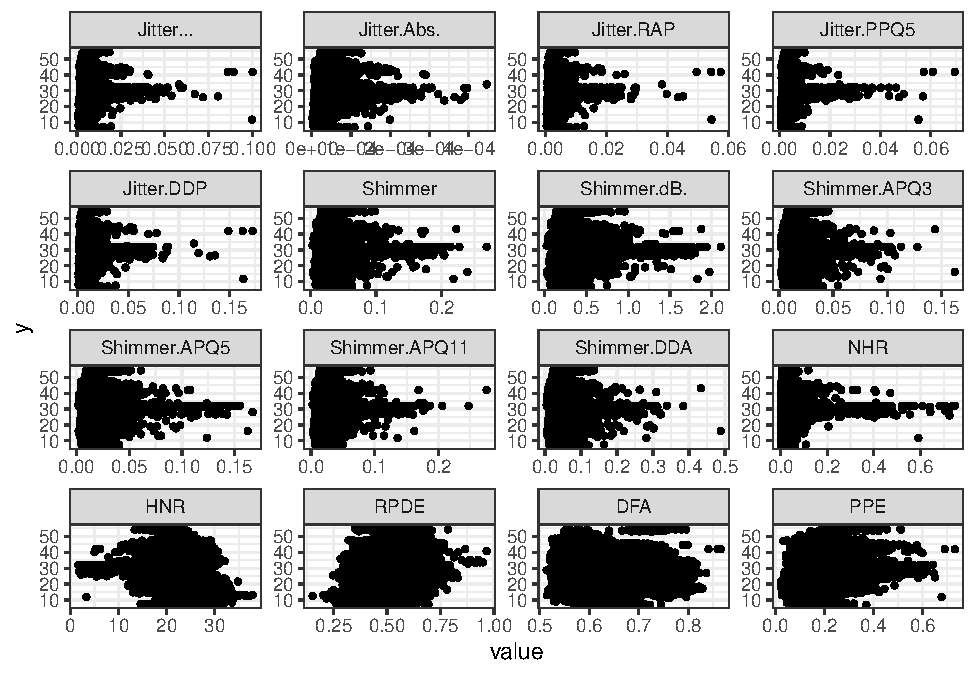
\includegraphics{Data_Exploration_files/figure-latex/unnamed-chunk-16-1.pdf}

Finally we compute the correlations among the covariates

\begin{Shaded}
\begin{Highlighting}[]
\NormalTok{cor\_cov }\OtherTok{\textless{}{-}} \FunctionTok{cor}\NormalTok{(dat[, }\DecValTok{7}\SpecialCharTok{:}\DecValTok{22}\NormalTok{], }\AttributeTok{method =} \StringTok{\textquotesingle{}spearman\textquotesingle{}}\NormalTok{)}
\FunctionTok{library}\NormalTok{(corrplot)}
\end{Highlighting}
\end{Shaded}

\begin{verbatim}
## corrplot 0.94 loaded
\end{verbatim}

\begin{Shaded}
\begin{Highlighting}[]
\FunctionTok{corrplot}\NormalTok{(cor\_cov)}
\end{Highlighting}
\end{Shaded}

\includegraphics{Data_Exploration_files/figure-latex/unnamed-chunk-17-1.pdf}

\begin{Shaded}
\begin{Highlighting}[]
\FunctionTok{corrplot.mixed}\NormalTok{(cor\_cov, }\AttributeTok{tl.col =} \StringTok{\textquotesingle{}black\textquotesingle{}}\NormalTok{, }\AttributeTok{insig =} \StringTok{\textquotesingle{}blank\textquotesingle{}}\NormalTok{, }\AttributeTok{tl.pos =} \StringTok{\textquotesingle{}lt\textquotesingle{}}\NormalTok{, }\AttributeTok{number.cex =} \FloatTok{0.5}\NormalTok{)}
\end{Highlighting}
\end{Shaded}

\includegraphics{Data_Exploration_files/figure-latex/unnamed-chunk-17-2.pdf}

\hypertarget{references}{%
\paragraph*{References}\label{references}}
\addcontentsline{toc}{paragraph}{References}

\hypertarget{refs}{}
\begin{CSLReferences}{1}{0}
\leavevmode\vadjust pre{\hypertarget{ref-tsanas2009accurate}{}}%
Tsanas, Athanasios, Max Little, Patrick McSharry, and Lorraine Ramig.
2009. {``Accurate Telemonitoring of Parkinson's Disease Progression by
Non-Invasive Speech Tests.''} \emph{Nature Precedings}, 1--1.

\end{CSLReferences}

\end{document}
